\documentclass{beamer}
\usepackage{graphicx}
\usepackage[ngerman]{babel}
\usepackage{amsmath,amssymb,amstext}
\usepackage[utf8]{inputenc}
\usepackage{array}
\usepackage{listings}
\usepackage{pgf}
\usepackage{tikz}
\usepackage{color}
\usepackage{colortbl}
\usepackage{picture,xcolor}
\usepackage{beamerthemesplit}
\usepackage{pgf}
\usepackage{listings}
\usepackage{bbm}
\usepackage{array}
\usepackage{mathptmx}
\usepackage{setspace}
\usepackage{comment}
\usepackage[absolute,overlay]{textpos}
\usepackage{txfonts}

\newcolumntype{a}{>{\columncolor{amber!90}}c}
\newcolumntype{r}{>{\columncolor{structure.bg!80}}l}
\newcolumntype{g}{>{\columncolor{gray!30}}c}

\usetikzlibrary{angles,arrows,shapes,snakes,automata,backgrounds,petri,3d,calc,patterns,quotes}

\newcommand{\dist}{\operatorname{d}}
\newcommand{\ch}{\textcolor{white}{\checkmark}}
\newcommand\vneq{\mathrel{\ooalign{$=$\cr\hidewidth$|$\hidewidth\cr}}}

\setbeamercolor{button}{bg=structure.bg, fg=structure.fg}



\newcommand{\figB}{\parbox{0.5cm}{\centering\begin{tikzpicture}[scale=0.34] %Kugel
		\draw (-1,0) arc (180:360:1cm and 0.3cm);
		\draw[dashed] (-1,0) arc (180:0:1cm and 0.3cm);
		\draw (0,1) arc (90:270:0.3cm and 1cm);
		\draw[dashed] (0,1) arc (90:-90:0.3cm and 1cm);
		\draw (0,0) circle (1cm);
		\shade[ball color=gray!10!white,opacity=0.20] (0,0) circle (1cm);
		\end{tikzpicture}} \hspace{0.25cm}}

% ------ environments
\newenvironment<>{prop}[1]{%
	\begin{block}{Proposition #1}}{\end{block}}
\newenvironment<>{cor}[1]{%
	\begin{block}{Corollary #1}}{\end{block}}
\newenvironment<>{thm}[1]{%
	\begin{block}{Theorem #1}}{\end{block}}  
\newenvironment<>{conj}[1]{%
	\begin{block}{Conjecture #1}}{\end{block}}
\newenvironment<>{lemma}[1]{%
	\begin{block}{Lemma #1}}{\end{block}}
\newenvironment<>{rem}[1]{%
	\setbeamercolor{block title}{fg=white,bg=uos-red}%
	\begin{block}{Remarks #1}}{\end{block}}
\newenvironment<>{not}[1]{%
	\begin{block}{Notation #1}}{\end{block}}


%\usefonttheme[onlymath]{serif}
\usepackage{concmath}


\lstset { %
	language=C++,
	backgroundcolor=\color{black!5}, % set backgroundcolor
	basicstyle=\footnotesize,% basic font setting
}
%\lstMakeShortInline[columns=fixed]|


% ------ theme
\usetheme[wave,sbgpic,nosections,frametitlecolored,progbar,cyclist,noframenumber]{SBG}

\setbeamercolor{itemize subitem}{fg=structure.bg!89!yellow}
\setbeamertemplate{itemize subitem}{\color{structure.bg!89!yellow}$\blacktriangleright$}



\newtheorem{beme}{Bemerkung}[section]

\title[BACHELOR PROJECT]{\bf \vspace{1cm} Erzeugung orthogonaler Transformationen mittels Strukturen aus optimierten Givens-Rotationen}
\author[DAVIDOUSKAYA]{\footnotesize MARYIA DAVIDOVSKAYA}
%\author[DAVIDOUSKAYA]{DAVIDOUSKAYA \vspace{1cm}}
\date{27. Jänner 2020}

\setcounter{tocdepth}{4}

\begin{document}
	%\usefont{T1}{futs}{m}{n}	
	
	
	%\AtBeginSubsection[]
	%{
	%	\begin{frame}<beamer>
	%		\frametitle{\figA Content}
	%		\tableofcontents[currentsection,currentsubsection,hideothersubsections]
	%	\end{frame}
	%}
	
	
	\frame[plain]{
		\titlepage
	}
	
	
	%\AtBeginSection[]
	%{
	%	\begin{frame}<beamer>
	%		\frametitle{\figA Content}
	%		\tableofcontents[currentsection,hideothersubsections]
	%	\end{frame}
	%}
	
%%%%%%%%%%%%%%%%%%%%%%%%%%%%%%%%%%%%%%%%%%%%%%%%%%%%%%%%%
%														%
%         			PROJECT								%
%														%
%%%%%%%%%%%%%%%%%%%%%%%%%%%%%%%%%%%%%%%%%%%%%%%%%%%%%%%%%
\section{M. DAVIDOVSKAYA}
\subsection{}
\frame{
	\frametitle{}
	\begin{itemize}
    \item Es geht nun darum, die $\alpha$-Parameter durch Optimierung zu finden, sodass das Ergebnis der nacheinander ausgeführten Givens-Rotationen für gewisse Eingangssignale gewisse Werte annimmt.
    \end{itemize}
}
\frame{
	\frametitle{Signal}
	\begin{itemize}
    \item (...x[$\num{-2}$],\overbrace{x[$\num{-1}$],x[0],x[1],x[2]},x[3]...)  $\in$ $\mathbb{C}$
   
    %\item \hspace{1,3cm} $\bowtie$ \hspace{0,2cm} $\bowtie$ \hspace{0,3cm} $\bowtie$
    
     \item hat linke Grenze und rechte Grenze (-1,2)
      \item index = index - indexLG
     \end{itemize}
}
\frame{
	\frametitle{Komplexe Zahlen}
	\begin{itemize}
    \item Zahl besteht aus zwei Komponenten:Real-und Imaginärteil
    	\begin{itemize}
     \item  z = a + ib,wobei i^2=-1
   \end{itemize}
    \end{itemize}
}


\frame{
	\frametitle{Givens-Rotation}
	\begin{itemize}
    \item In der linearen Algebra ist eine Givens-Rotation (nach Wallace Givens) eine Drehung in einer Ebene, die durch zwei Koordinaten-Achsen aufgespannt wird. Manchmal wird dies auch als Jacobi-Rotation (nach Carl Gustav Jacobi) bezeichnet.
    \end{itemize}
}
\frame{
	\frametitle{Geometrische Ansicht}
	\begin{itemize}
    \item Um die Givens-Rotation zu verstehen,ist es von Vorteil,das Prinzip der allgemeinen Rotation von Vektoren in der Ebene zu kennen.Soll ein Punkt P \begin{pmatrix}x\\y\end{pmatrix} um einen Winkel $\phi$ um den Koordinatenursprung rotiert werden,muss die Rotationsmatrix  G$\phi$ bestimmt werden.

	\end{itemize}
}
\frame{
	\frametitle{Allgemeine Rotation von Punkten}

   	\begin{center}
		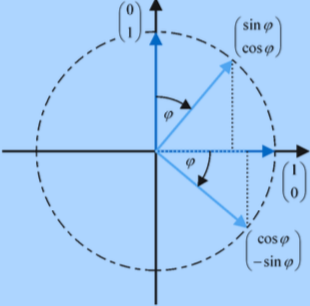
\includegraphics[width=0.50\textwidth]{givens.png}\\
    \end{center}
}
\frame{
	\frametitle{Beschreibung}
	\begin{itemize}
	 \item  Eine Drehung im $\text{R}^2$ um den Winkel $\phi$ ist durch eine orthogonale Rotationsmatrix  G$\phi$  charakterisiert:
    \item   G$\phi$ =  \begin{pmatrix}c & s\\-s & c\end{pmatrix}
    wobei c = cos($\phi$) und s = sin($\phi$) 
    \item $\phi$ $\in$ [0,2$\pi$]
    \end{itemize}
}
\frame{
	\frametitle{Beschreibung}
	\begin{itemize}
	\item  \begin{pmatrix}x[2]\\x[4]\end{pmatrix} =  \begin{pmatrix}c & s\\-s & c\end{pmatrix} $\cdot$\begin{pmatrix}x[2]\\x[4]\end{pmatrix}
    \item  temp = x[2] $\cdot$ c + x[4] $\cdot$ s;
    \item  x[4] = x[4] $\cdot$ c - x[2] $\cdot$ s;
    \item  x[2] = temp;
    \end{itemize}
}
\frame{
	\frametitle{Schicht}
	\begin{itemize}
	\item Eine Schicht von Givens-Rotationen hat nun folgende Form:
	 \begin{itemize}
	 \item  $\ $[a,b]+c $\{$0...d$\}$+e$\{$0... f$\}$+g$\mathbb{Z}$ .
	  \end{itemize}
	  \item Das heißt,dass [a,b] eine Givens-Rotation der Schicht ist,
	  aber auch alle [a+ic+ je + kg , b + ic + je + kg], wobei i = 0 . . . d , j = 0 . . . f , und k  $\in$  $\mathbb{Z}$ 
    \end{itemize}
}
\frame{
	\frametitle{Beispiel}
	\begin{itemize}
    \item  $\ $[0,2]+1$\{$0...1$\}$+4$\{$0...1$\}$+8$\mathbb{Z}$
    \item  (...,[\num{-4},\num{-2}],[\num{-3},\num{-1}],[0,2],[1,3],[4,6],[5,7],[8,10],[9,11],...).
    \end{itemize}
}
\frame{
	\frametitle{Schicht}
	\begin{itemize}
	\item \hspace{1,6cm} - g  \hspace{5,7cm} + g
	\item  ($\overbrace{...,[\num{-4},\num{-2}],[\num{-3},\num{-1}]}$,$\overbrace{[0,2],[1,3],[4,6],[5,7]}$,$\overbrace{[8,10],[9,11],...}$).
    \item Es sollen alle mit gleichem i und j den selben Rotationsparameter α besitzen.
    \item  Im Beispiel ist also $\alpha$[0,2] = $\alpha$[8,10], und auch $\alpha$[\num{-3},\num{-1}] = $\alpha$[5,7], usw. 
    \item Die Schicht hat also nur vier $\alpha$-Parameter.
    \item Die Rotationen einer Schicht sollten sich nicht überlappen.
    \end{itemize}
}
\frame{
	\frametitle{Scheme}
	\begin{itemize}
    \item Ein Schema von Givens-Rotationen ist einfach eine Sequenz von Schichten.
   \end{itemize}
}
\frame{
	\frametitle{Eingangssignal}
	\begin{itemize}
	\item Das Eingangssignal hat immer die Form:
     x[t]= $\text{e}^i^\Theta^t$, also ein Signal mit Frequenz $\Theta$ mit  0 \leq \ $\Theta$ \leq \ $\pi$,dabei ist e $\approx$ 2,71828
    die Euler’sche Zahl.
     \item{ Form der Darstellung, die durch die Euler'sche Formel gegeben ist.}
      \begin{itemize}
        \item{$\text{e}^i^\Theta^t$ = cos($\Theta$t) + isin($\Theta$t)}
      
      \end{itemize}
   \item  Polardarstellung von z bezeichnet man als:
    \begin{itemize}
     \item  z = r cos($\Theta$t) + i r sin( $\Theta$t)= r$\text{e}^i^\Theta^t$, r=$|z|$
     
       \end{itemize}
 \item polar(1.0,$\Theta$t)
    \end{itemize}
}
\frame{
	\frametitle{Das gewünschte Ergebnis}
	\begin{itemize}
    \item  Das gewünschte Ergebnis soll auf folgende Weise definiert werden:
    	 \begin{itemize}
	 \item y_{\Theta}[t]= \begin{cases} B_{t,0}e^i^{\beta t,0}^\Theta \qquad  0 \leq \ \Theta \leq \ \Theta_{t,0} \\ B_{t,1}e^i^{\beta t,1}^\Theta \qquad  \Theta_{t,0} \leq \ \Theta \leq \ \Theta_{t,1}\\ B_{t,2}e^i^{\beta t,2}^\Theta \qquad  \Theta_{t,1} \leq \ \Theta \leq \ \pi\end{cases}

	  \end{itemize}
   \end{itemize}
}
\frame{
	\frametitle{Fehlerfunktion}
	\begin{itemize}
    \item Es sei nun  ${\^x_\Theta[t]}$ das durch die  Givens-Rotationen transformierte  Eingangssignal. 
      \item Die Fehlerfunktion ist gegeben  durch
	 	\begin{itemize}
     \item E =  ${\int_{0}^{\pi}\sum\limits_{t}|\^x_\Theta[t] - y_\Theta[t] |^2 d\Theta}$
   \end{itemize}
   \item 
wobei über alle bei ${y_\Theta[t]}$ angegebenen t summiert wird und das Integral durch Summierung in kleinen (konfigurierbaren) Schritten von $\Theta$ implementiert werden soll.
   \end{itemize}
}
\frame{
	\frametitle{Die Gnu Scientific Library}
	\begin{itemize}
    \item Die Fehlerfunktion E soll nun durch Variieren der $\alpha$-Parameter minimiert werden.
    \item Dazu sollte die Gnu Scientific Library verwendet werden.
    \item Und zwar soll eine Methode zur mehrdimensionalen Minimierung mit Ableitungen verwendet werden
   \end{itemize}
}
\frame{
	\frametitle{Die Ableitungen}
	\begin{itemize}
    \item Dazu müssen die Ableitungen gebildet werden
    \begin{itemize}
    \item  ${\frac{dE}{d\alpha_{[a,b]}} = \int_{0}^{\pi}\sum\limits_{t}2\mathbb{R}\Biggl( (\^x_\Theta[t] - y_\Theta[t])\frac{\overline{d\^x_\Theta[t]}}{d\alpha_{[a,b]}}\Biggr)}$
   \end{itemize}
   \item wobei $\mathbb{R}$ der Realteil ist
   \end{itemize}
}
\frame{
	\frametitle{Die Ableitungen}
	\begin{itemize}
    \item $\frac{d\^x_\Theta[t]}{d\alpha_{[a,b]}}$ einfach berechnet
    werden kann, indem man die Rotation [a,b] durch
    	\begin{itemize}
    	 \item  \begin{pmatrix}x[a]\\x[b]\end{pmatrix} =  \begin{pmatrix}-s & c\\-c & -s\end{pmatrix} $\ast$\begin{pmatrix}x[a]\\x[b]\end{pmatrix} ersetzt
    	  \end{itemize}
    	   \item alle anderen Rotationen gleich lässt, und außerdem in der gleichen Schicht alle anderen x-Werte auf 0 setzt. Alle anderen Schichten werden unverändert berechnet.
   \end{itemize}
}


 
 %\frame{
%	\frametitle{Fazit}
 %  \begin{center}
 %		\begin{tabular}{||c c c c||} 
 %			\hline
 %			Kombinationen & 10 Paket & 100 Paket & 10000 Paket \\ [0.5ex] 
 %			\hline\hline
 %			c $\rightarrow$ c & 0.0002 & 0.002 & 0.14 \\ 
 %			\hline
 %			c $\rightarrow$ java & 0.0001 & 0.001 & 0.19 \\
 %			\hline
 %			java $\rightarrow$ java & 0.0004 & 0.005 & 0.5 \\
 %			\hline
 %			java $\rightarrow$ c & 0.0006 & 0.004 & 0.3 \\
 %			\hline
%		\end{tabular}
%	\end{center}
%}
% \documentclass[12pt]{beamer}
% %\documentclass[12pt,draft]{article}
% \usepackage{graphicx}
% \usepackage[ngerman]{babel}
% \usepackage{amsmath,amssymb,amstext,latexsym}
% \usepackage[utf8]{inputenc}
% \usepackage{tikz}
% \usepackage{color}
% \usepackage{xcolor}
% \usepackage{colortbl}
% \usepackage{picture,xcolor}
% \usepackage{beamerthemesplit}
% \usepackage{pgf}
% \usepackage{bbm}
% \usepackage{array}
% \usepackage{mathptmx}
% \usepackage{verbatim}
% \usepackage{listings}
% \usepackage{hyperref}
% \usepackage[shortlabels]{enumerate}
% \usepackage[official]{eurosym}

% \usepackage{comment}
% \usepackage[absolute,overlay]{textpos}
% \usepackage{txfonts}

% \newcolumntype{a}{>{\columncolor{amber!90}}c}
% \newcolumntype{r}{>{\columncolor{structure.bg!80}}l}
% \newcolumntype{g}{>{\columncolor{gray!30}}c}
% \setbeamercolor{button}{bg=structure.bg, fg=structure.fg}
% \setbeamercolor{local structure}{fg=structure.bg}
% \usepackage{concmath}
% \usetheme[sbgpic,progbar,noframenumber,subsectionpage,football]{SBG}
% \setbeamertemplate{itemize subitem}{\color{structure.fg}$\blacktriangleright$}
% \newtheorem{beme}{Bemerkung}[section]

% \title[\hspace{1cm} Netze und verteilte Systeme PS:G2]{\bf Erzeugung orthogonaler Transformationen mittels Strukturen aus optimierten Givens-Rotationen}
% \author[DAVIDOUSKAYA]{\footnotesize MARYIA DAVIDOVSKAYA\vspace{2mm}}
% \date{\vspace{5mm} WS 2019}

% \setcounter{tocdepth}{4}
% \begin{document}
% \frame[plain]{
%     \titlepage
% }  
\end{document}
